In this chapter, we will introduce the two solving approaches that we explored. Solving can be performed using already computed-paths or a subgraph defined by paths.

Solving in both cases is basically performed using the encoding defined in Listing~\ref{lst:solver}.

\begin{minipage}[H]{\linewidth}
\begin{lstlisting}[style=mystyle, caption={Encoding of final solver}, label={lst:solver}, numbers=left, ,escapechar=|]
    time(1..horizon).

    at(R,P,0) :- start(R,P).

    { move(R,U,V,T) : nedge(U,V)} 1 :- agent(R), time(T).

    at(R,V,T) :- move(R,_,V,T).
            :- move(R,U,_,T), not at(R,U,T-1).

    at(R,V,T) :- 
        at(R,V,T-1), 
        not move(R,V,_,T), 
        time(T).

    :- {at(R,V,T)}!=1, agent(R), time(T).|\label{line:one_position_at_a_time}|

    :- { at(R,V,T) : agent(R) }  > 1, nvertex(V), time(T).
    :- move(_,U,V,T), move(_,V,U,T), U < V.

    goal_reached(R) :- at(R,V,horizon), goal(R,V). |\label{line:ipf_goal_reached}|

    #maximize{1,R : goal_reached(R)}. |\label{line:maximize_goal_reached}|
\end{lstlisting}
\end{minipage}


This encoding is derived from the MAPF encoding illustrated in Listing~\ref{lst:base_mapf_encoding} with two significant modifications. The first modification involves the redefinition of movement predicates. Instead of relying on \(vertex/1\) and \(edges/2\), movement is now defined on \(nvertex/1\) and \(nedge/2\), which are generated from the encoding detailed in Listing~\ref{lst:converting_paths_to_subgraph}.

The second distinction is highlighted in lines~\ref{line:ipf_goal_reached} and~\ref{line:maximize_goal_reached}. Unlike classical MAPF, which either provides a complete solution or returns unsatisfiable if no solution exists, the solver in this context can produce a partial solution. This means that due to the steps taken to reduce the complexity MAPF problem, there is a possibility that the solver might not find a complete solution the way we defined it. However, it is possible to extend the algorithm to guarantee the solution by relaxing selected paths -- in the worse case, we relax all selected paths. Which correspond to classical MAPF solving. 


In order to highlight the differences between the two different kinds of solving approaches, we introduce an example in figure~\ref{fig:partial_solving_example}; a \(\tau\) result of IPF of a MAPF problem \(\mathcal{P}\).

\begin{figure}[H]
    \centering
    \caption{Example for solving approaches. Having a \(|\tau| = 3\) as result of IPF}\label{fig:partial_solving_example}
    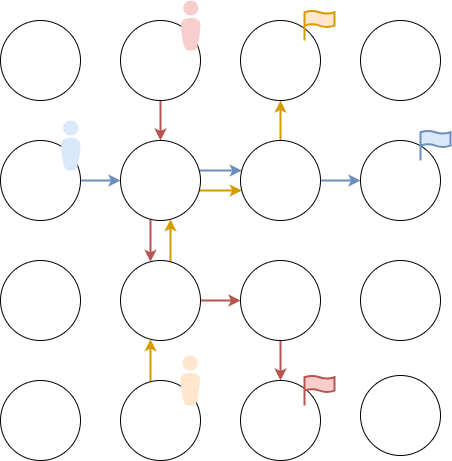
\includegraphics[width=9cm]{img/partial_solving_example.png}
\end{figure}




\section{Pre-computed paths}
As mentioned in the Path Selection section~\ref{sec:pathselection}, the output can vary based on the specified objective. In the context of the primary objective, which aims to construct a (partial) plan, we utilize the set of \textbf{selected paths} to generate \textbf{pre-computed paths}. This translation is achieved through the following rules:

\begin{minipage}[H]{\linewidth}
\begin{lstlisting}[style=mystyle]
    at(R,V,T) :- selected_path(R,I), at(R,I,V,T). |\label{line:selected_to_at}|
\end{lstlisting}
\end{minipage} 
\noindent Through line~\ref{line:selected_to_at}, we ensure that the selected paths are incorporated into the solution. Conversely, for agents without a selected path, the encoding is employed to compute their paths.

\begin{figure}[H]
    \centering
    \caption{Possible output for Path Selection \& Pre computed paths}\label{fig:pre_computed_path_solving}
    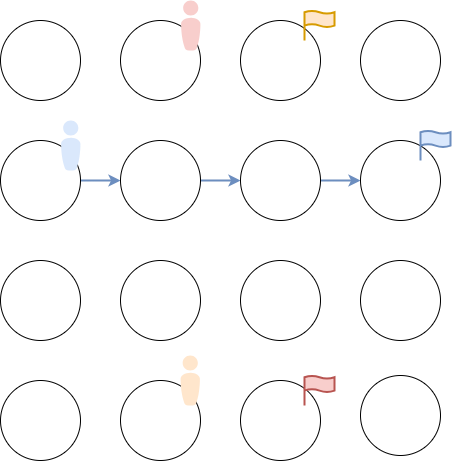
\includegraphics[width=9cm]{img/pre_computed_path_solving.drawio.png}
\end{figure}

Figure~\ref{fig:pre_computed_path_solving} describes a partial plan \(\hat{\Pi}\) where only blue agent has a path. Partial Solving now computes path for the two remaining agents, which is, hopefully easier than computing paths for the all three. In the example outlined in figure~\ref{fig:pre_computed_path_solving}, the solving requires a makespan of five.

\section{Subgraph}

The second objective described in Section~\ref{sec:pathselection} aims to create a subgraph in order to reduce the size of the problem. From the paths in Figure~\ref{fig:partial_solving_example}, we obtain the subgraph shown in Figure~\ref{fig:subgraph_solving}.

\begin{figure}[H]
    \centering
    \caption{Example for solving approaches. Having a \(|\tau| = 3\) as result of IPF}\label{fig:subgraph_solving}
    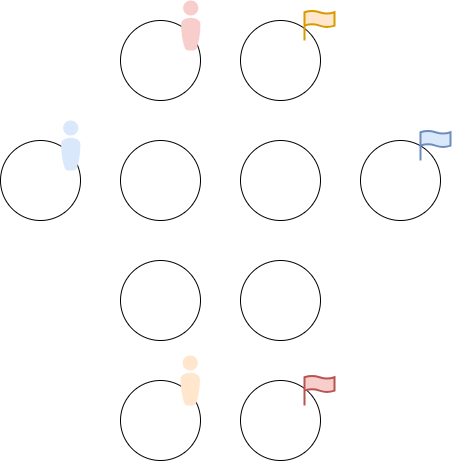
\includegraphics[width=9cm]{img/subgraph_solving.png}
\end{figure}

Contrary to pre-computing path, we aim to reduce the size of the graph the agents can move on. Applying MAPF on the problems described in figure~\ref{fig:subgraph_solving} can find a solution with a makespan of 4.

The two approaches presented can be used as one. 

\subsection{Subgraphs Extension Strategies}

In practice, the subgraph solving approach seems to not be enough to fully solve instances; the agents seem to require too many additional time steps in order to ``solve conflict''. Thus, we introduce two strategies in order to extend subgraphs. 

\subsubsection{Corridor}

The corridor strategy~\cite{surynek2023candidate} is engineered to augment the subgraph-solving process by incorporating neighboring vertices and their associated edges directly into the sub-graph. Corridors can vary in size, allowing for different levels of expansion. Figure~\ref{img:corridor} illustrates a corridor of size one.

\begin{figure}[H]
    \centering
    \caption{Example of corridor}\label{img:corridor}
    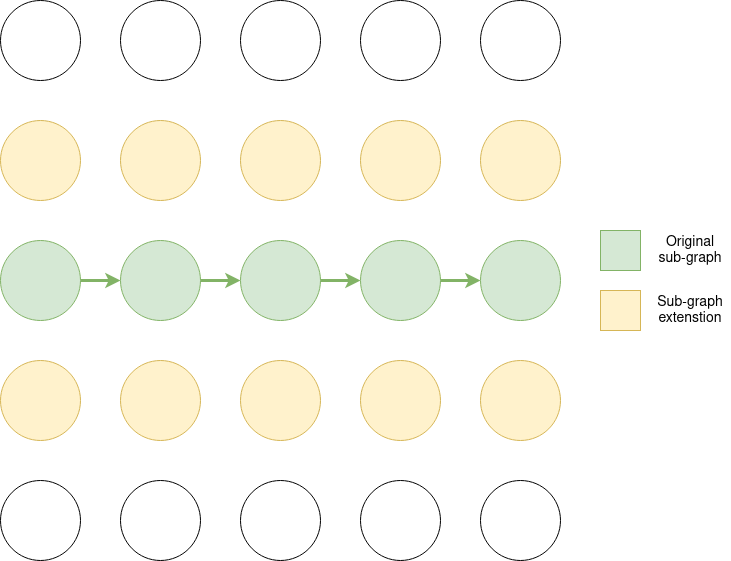
\includegraphics[width=\widthimg]{img/corridor.drawio.png}
\end{figure}

The following encoding in Listing~\ref{lst:corridor_encoding} describe how corridors for paths can be computed.

\begin{minipage}[H]{\linewidth}
\begin{lstlisting}[style=mystyle, caption={Corridor extension encoding}, label={lst:corridor_encoding}]
    #const corridor_level = 2.

    corridor(V,0) :- selected_path_for_corridor(R,I), at(R,I,V,_).
    
    corridor(V,K+1) :- 
        K < corridor_level,
        corridor(U,K),
        edge(U,V).

    nvertex(V) :- corridor(V,_).
\end{lstlisting}
\end{minipage}

Predicate \(selected\_path\_for\_corridor/2\) highlights a path that requires a corridor extension.

With a sufficiently large \(k\), the entire graph can be covered; using a large corridor could essentially revert the problem back to a classical MAPF scenario.

In practice, corridors are created only for paths involved in conflicts, and a choice can be made to create corridors for only one of the two agents involved in a conflict.

\subsubsection{Diamond}

The diamond extension strategy involves expanding the sub-graph by incorporating diamond-shaped arrangements of vertices around conflicting vertices. As illustrated in figure~\ref{img:diamond}, various levels of diamond extension can be applied, each increasing the size of the sub-graph and thereby expanding the possibilities for conflict resolution.

\begin{figure}[H]
  \centering
  \caption{Example of diamond of size 1 and 2}\label{img:diamond}
  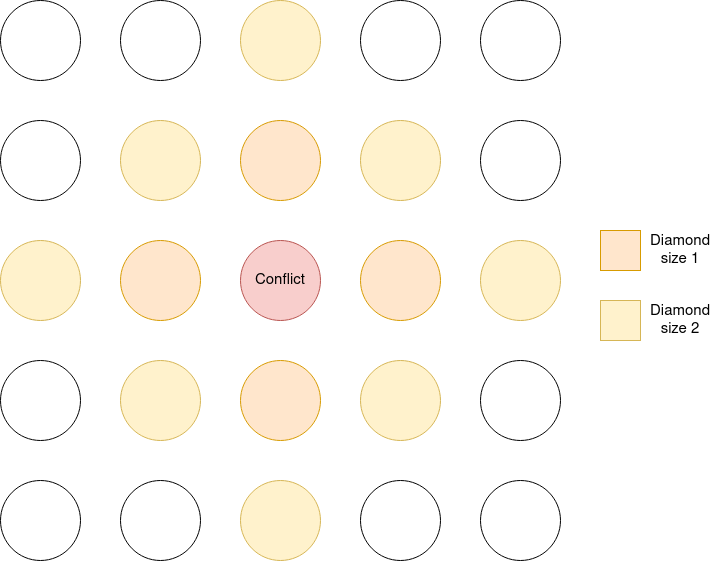
\includegraphics[width=\widthimg]{img/diamond.drawio.png}
\end{figure}


The encoding in Listing~\ref{lst:corridor_encoding} describes how diamonds are computed. As for corridors, the predicate \(selected\_vertex\_for\_diamond/1\) highlight a vertex that requires a diamond extension. In practice, we apply diamond extension on every conflict induced by the set of paths composing the subgraph. 

\begin{minipage}[H]{\linewidth}
\begin{lstlisting}[style=mystyle, caption={Diamond extension encoding}, label={lst:diamond_encoding}]
    #const diamond_level = 2.
    diamond(V,0) :- selected_vertex_for_diamond(V).
    
    diamond(V,S+1) :- 
        diamond(U,S), 
        S<diamond_level, 
        edge(U,V).
    
    nvertex(V) :- diamond(V,_).
\end{lstlisting}
\end{minipage}

